\documentclass[8pt]{beamer}

\usepackage[utf8]{inputenc}
\usepackage{default}
\usepackage{hyperref}
\usepackage{textpos}
\usepackage{verbatimbox}
\usetheme{Copenhagen}

\title{Blockchains}
\subtitle{Cryptocurrencies and Consortium Blockchains}
\author{Tero Keski-Valkama}
\institute{
\includegraphics[height=1.4cm]{CybercomG_logo_Classic_RGB.png}}
\date{2017-01-19}

\addtobeamertemplate{frametitle}{}{%
\begin{textblock*}{100mm}(10.95cm,-0.8cm)

\includegraphics[height=0.8cm]{cybercom-blue.png}
\end{textblock*}}


\begin{document}

\frame{\titlepage}
 
\begin{frame}
\frametitle{What is Blockchain}

\begin{itemize}
 \item Blockchain is a collection of cryptotechnologies to achieve a distributed consensus about immutable, additive data in an untrusted environment.
 \begin{enumerate}
  \item Blockchain is a sequence of records, or blocks, so that each block contains a hash digest of the previous block (which recursively contains the hash digest of the previous block and so on).
  \item A consensus mechanism with rules to determine which blocks are accepted to be the next block in the blockchain. Many solutions such as proof-of-work, proof-of-stake, proof-of-burn,
        Practical Byzantine Fault Tolerance, and hybrids.
  \item A discovery and broadcast infrastructure to relay transactions and blocks to peers and miners.
  \item Application-specific public key or other cryptography to prove identities of parties in transactions, wallets and so on.
  \item Microcode used to define the transaction semantics or smart contracts, such as \href{https://en.bitcoin.it/wiki/Script}{Bitcoin Script}, \href{http://solidity.readthedocs.io/en/latest/}{Solidity}
        or \href{https://github.com/IBM-Blockchain/learn-chaincode}{Chaincode}.
 \end{enumerate}
 \item In blockchain, a single valid block can be used to validate the whole chain of blocks to deep history so that anyone can make sure that nothing has been altered in the stored data,
       by checking that the hashes of the previous block always matches the content of the previous block.
 \item The consensus mechanism offers guarantees that all parties have a converging view in the blockchain regarding what is valid and what is not. It prevents changing the history and
       that the whole blockchain integrity is guaranteed.
\end{itemize}

\end{frame}

\begin{frame}
\frametitle{There Shall Be No Blockchain But Bitcoin}

\begin{figure}[tb]
 \centering
 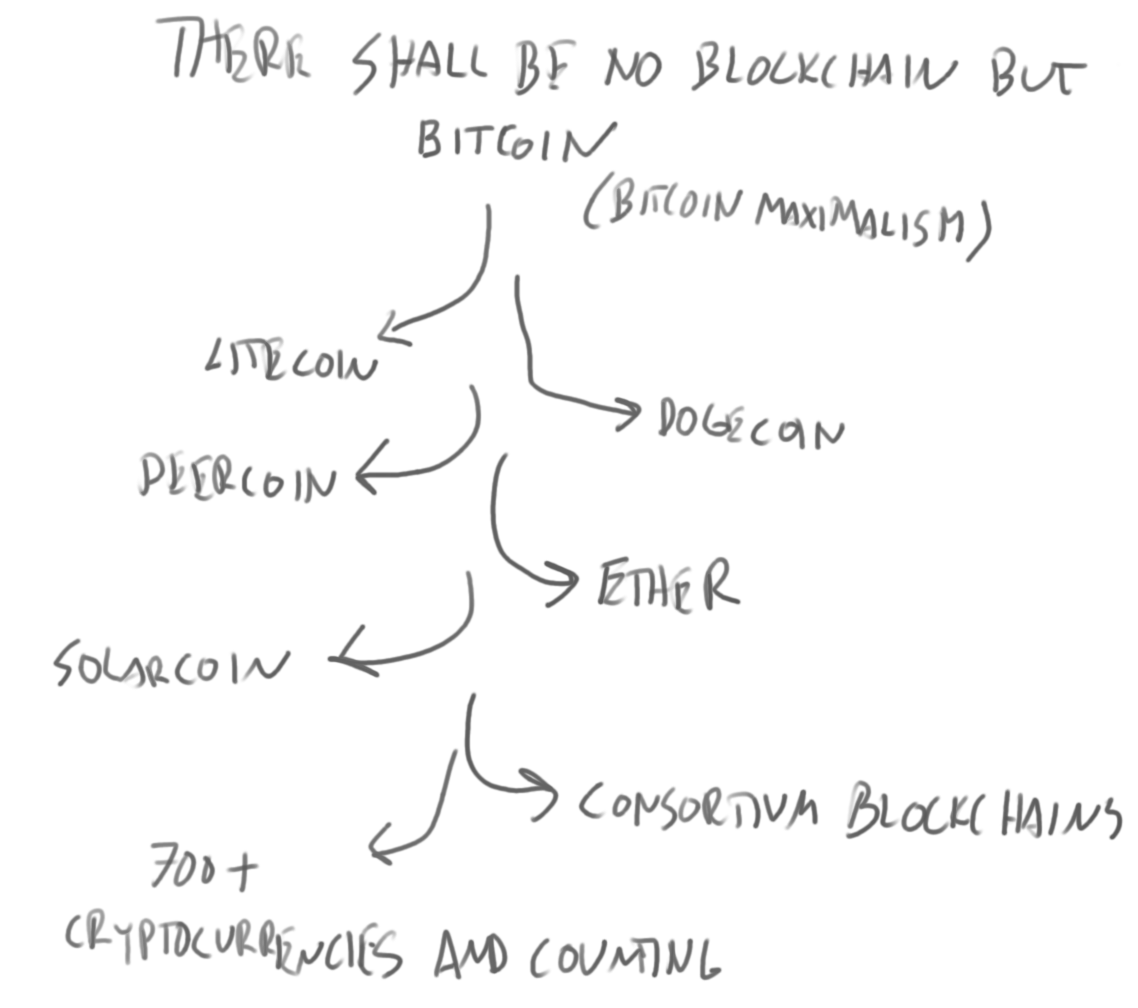
\includegraphics[width=8 cm,keepaspectratio=true]{./blockchain_images/only_bitcoin.png}
 \caption{Bitcoin Maximalism vs. The Reality}
\end{figure}

\end{frame}

\begin{frame}
\frametitle{Comparison of Associated Technologies}

\begin{tabular}{| l | c | c | c |}
\hline
 & \shortstack{Distributed \\ Database} & \shortstack{Consortium \\ Blockchain} & \shortstack{Cryptocurrency \\ Blockchain} \\
\hline
\shortstack{Consensus \\ mechanism} & \shortstack{Simple \\ parallel consistency} & \shortstack{Byzantine \\ Fault Tolerance} & \shortstack{Proof-of-Work, \\ Proof-of-Stake, \\ Proof-of-Burn \\ or a hybrid} \\
\hline
\shortstack{Requires \\ a cryptocurrency} & & & X \\
\hline
\shortstack{Open ecosystem \\ of untrusted peers} & & & X \\
\hline
\shortstack{Peers validate \\ each other's actions} & & X & X \\
\hline
\shortstack{Access \\ centrally managed} & X & X & \\
\hline
\end{tabular} 

\end{frame}

\begin{frame}
\frametitle{Comparison of Consensus Methods}

\begin{figure}[tb]
 \centering
 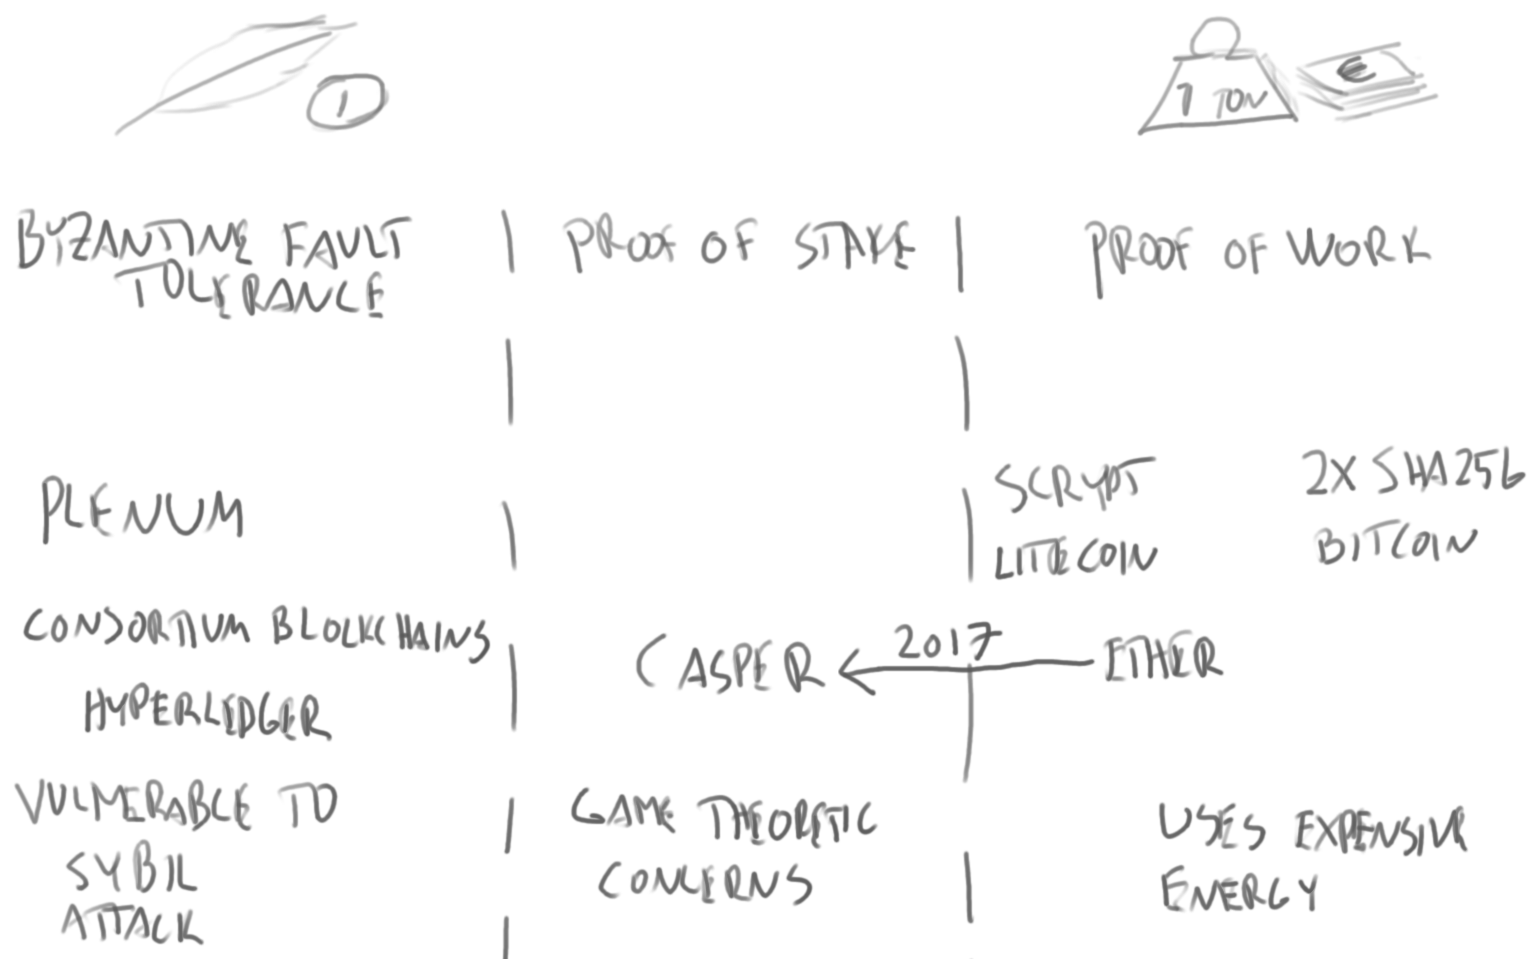
\includegraphics[width=8 cm,keepaspectratio=true]{./blockchain_images/comparison.png}
 \caption{Consensus Methods}
\end{figure}

\end{frame}

\begin{frame}
\frametitle{Consensus Mechanisms}

\begin{itemize}
 \item Consensus is inherently a game theoretic concept in Byzantine systems, because the peers can try to cheat.
 \item In open ecosystems it must be made economically infeasible to break the rules or the goals of the system. This leads to the requirement of having a cryptocurrency built into the system.
       In practice, a validating peer gains cryptocurrency for processing transactions, and this cryptocurrency only has value if the whole system works.
 \item A Bitcoin data center is under construction in China designed to consume 135 MW of power. This is for 7 transactions per second for the whole Bitcoin network for the current block size limit of 1 MB.
       The Chinese data center energy consumption is roughly 5 kilograms of coal equivalent per second.
 \item In closed consortiums, it is feasible to get rid of peers behaving incorrectly, so expensive proof-operations can be avoided.
\end{itemize}
\end{frame}

\begin{frame}
\frametitle{Proof of Work}

\begin{itemize}
 \item Proof-of-work algorithms include for example Bitcoin double SHA256, or Litecoin Scrypt.
\end{itemize}


\end{frame}

\begin{frame}
\frametitle{Proof of Stake}

\begin{itemize}
 \item Proof-of-Stake is a proposed alternative to energy wasting Proof-of-Work. Instead of proving you have done work, you prove you own a number of coins.
 \item Generally, for each block each coin gets a random chance of determining the next block.
 \item Game theoretic worries: If the miners have no stake, why would they play fair?
 \item Proof-of-work algorithms include for example Bitcoin double SHA256, or Litecoin Scrypt.
\end{itemize}

\end{frame}

\begin{frame}
\frametitle{Byzantine Fault Tolerance}
\begin{itemize}
 \item Byzantine Fault Tolerance refers to a general game theoretic mathematical problem where distributed parties try to achieve consensus in spite of unreliable messaging and hostile actors.
 \item There are several algorithms and implementations with different characteristics.
 \item Practical Byzantine Fault Tolerance algorithm useful for consortium blockchains, but cannot be used for open blockchains.
 \item Byzantine Fault Tolerance algorithms do not generally consider an open system where new actors can join at will, and therefore they implicitly assume a kind of a Proof-of-Stake through association to the group.
 \item These algorithms generally need a centralized identity management to prevent a Sybil attack. Although it could be said that the centralized identity manager could freely perform a Sybil attack in these systems.
\end{itemize}

\end{frame}

\begin{frame}
\frametitle{Comparison of Chaincode Languages}

\begin{figure}[tb]
 \centering
 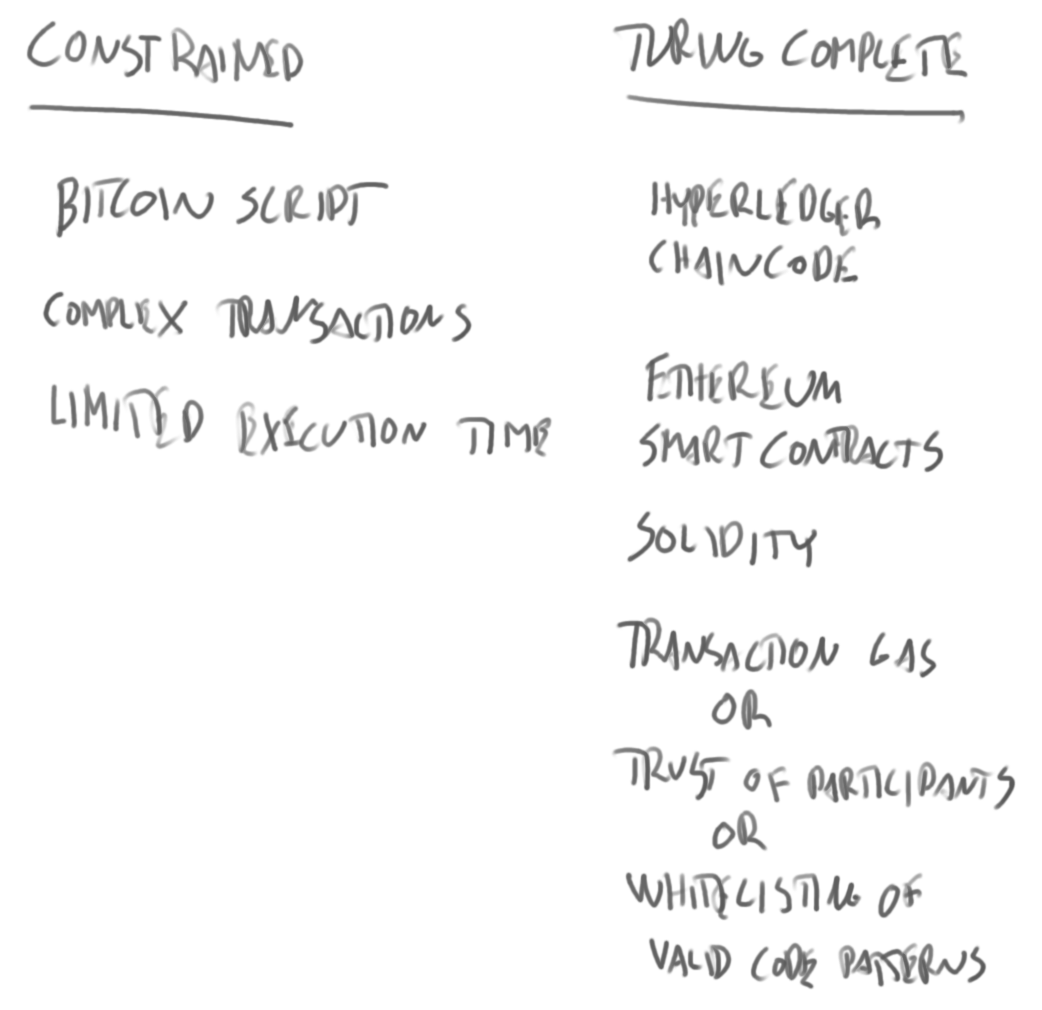
\includegraphics[width=6 cm,keepaspectratio=true]{./blockchain_images/chaincodes.png}
 \caption{Chaincode Languages}
\end{figure}

\end{frame}

\end{document}

